%% Template for a preprint Letter or Article for submission
%% to the journal Nature.
%% Written by Peter Czoschke, 26 February 2004
%%

\documentclass{nature}

%% make sure you have the nature.cls and naturemag.bst files where
%% LaTeX can find them

\bibliographystyle{naturemag}
\usepackage{color}

\title{Computer vision profiling of neurite outgrowth morphodynamic phenotypes}

%% Notice placement of commas and superscripts and use of &
%% in the author list

\author{Ludovico Fusco$^{1,6}$, Fethallah Benmansour$^{2. 6}$, Riwal Lefort$^{3, 6}$, Kevin Smith$^{4, 6}$, German Gonzales$^4$,  Catherina Barillari$^5$, Bernd Rinn$^5$, Francois Fleuret$^3$, Pascal Fua$^2$  \& Olivier Pertz$^1$}


%======================================================================
\begin{document}

\maketitle

\begin{affiliations}
 \item Institute for Biochemistry and Genetics, Dept. Biomedicine, University of Basel, Mattenstrasse 28, 4058 Basel, Switzerland
 \item 
 \item 
 \item 
 \item 
 \item 
\end{affiliations}


sdgdfgf d
%======================================================================
%% -*- mode: latex; mode: reftex; mode: flyspell; TeX-master: "top.tex"; -*-

%gg 20121023 - strengthened the findings
We present a fully automatic method  to track and quantify the morphodynamics of differentiating neurons  in fluorescence  time-lapse datasets.  Previous high-throughput studies are limited to static analysis or simple behavior. Our approach opens the door to rich dynamic analysis of complex cellular behavior in high-throughput time-lapse data. It is capable of  robustly detecting, tracking,  and segmenting all the  components of the neuron including the nucleus, soma, neurites, and filopodia. It was designed to be efficient enough to handle the massive amount of data from a high-throughput screen. Each image is processed in approximately two seconds on a notebook computer. To validate  our approach,  we analyzed over 500 neuronal differentiation videos from a small-scale RNAi screen. Our fully automated analysis of over 7,000 neurons quantifies  and  confirms with strong statistical significance static and dynamic behaviors that  had  been previously observed by biologists, but never measured. 

%Finally, we are first to
%analyze temporally the  behavior of neurons, leading to  findings not measurable
%through  state-of-the-art static  analysis. All  our findings  are statistically
%significant, with a p-value $\ll 0.05$.

%% We  present  a  fully  automatic  method to  track  and  quantify  the
%% morphodynamics of  differentiating neurons in  fluorescence time-lapse
%% datasets.     Our  approach is capable of robustly detecting,
%% tracking, and segmenting all the  components of the neuron including 
%% the nucleus, soma, neurites, and filopodia.  It is designed to be extremely efficient, capable of processing
%% each image in approximately two seconds on a conventional notebook
%% computer.  To validate our approach, we  analyzed  neuronal
%% differentiation videos in  which a set of genes  was perturbed using
%% RNA interference. Our analysis quantifes and confirms morphodynamic behaviors 
%% which had been previously observed by biologists but never measured.
%% Finally, we present new observations on the behavior of neurons made
%% possible by our analysis which could not be discovered through static analyis.


\begin{keywords}
Molecular and cellular screening; Image sequence processing; Fluorescence microscopy
\end{keywords}

%  whose
%measurements were not feasible on a large scale.  Finally, using our
%quantitative analysis we make

%our dynamic
%quantitative analysis allows us to  make new observations that are not
%visible to a human observer.


%% we  use it to  perform an siRNA  screen and
%% successfully reproduce the findings of~\cite{}, which was performed at
%% steady-state under less stressful conditions [OLVIER, HELP US SAY THIS
%%   MORE  ELOQUENTLY].   Finally, we  apply  our  approach  to make  new
%% observations   based  on  dynamic   quantitative  analysis   that  was
%% previously impossible.

%% While  previous efforts
%% have tracked the soma and nucleus,  our approach is the first to fully automatically track
%% and reconstruct the neurites as  they expand, branch and collapse, and
%% to dynamically detect fine filopodia structures.

%We present a method to analyze and extract statistics from large-scale
%video sequences  of in-vitro neurons.   Our system is able  to detect,
%track, segment  and reconstruct each individual neuron  present on the
%videos.   We show how  such system  can be  used to  find correlations
%between neuron behaviour and the proteins used to mutate them.

%high throughput automation

%confirms pre-existing findings

%yields new understandings about the dynamic morphologies

%efficient, tracks, segments, and tracks neurites


%======================================================================

%======================================================================
%% -*- mode: latex; mode: reftex; mode: flyspell; TeX-master: "top.tex"; -*-


The  process  of forming  functional  connections  between neurons  is
complex  and   dynamic.   Time-lapse  microscopy   has  revealed  that
differentiating  neurons undergo  a large  range of  dynamic processes
including cell body motility, filopodial dynamics, and repeated cycles
of  neurite growth  and  retraction.  Of  critical  importance is  the
process  by which  axons and  dendrites are  formed in  which a neurite
ceases retracting, extends a   long  distance, and  forms
a connection. Such  dynamic events are  governed by a  complex protein
network that  coordinates   dynamic functions 
within the cytoskeleton, membrane, etc.

Powerful tools such as 
RNA interference  (RNAi)
technology,  fluorescent  protein   labeling,  image  processing,  and
automated high-throughput  microscopy have  opened the door  for large
scale  perturbation studies to help investigate such processes. RNAi  screens have  already led  to novel
insights   into  a  number   of  cellular   processes  such   as  cell
migration~\cite{Bakal07}  and endocytosis~\cite{Collinet10}.  However,
limitations  in  image  processing  have  restricted  most
investigations to static image analysis.

Knowledge  of dynamics is  essential if we are  to understand
complex  processes such  as neuron  morphogenesis.  However, designing
algorithms to quantify dynamic  behaviors is challenging, and
automatic methods  have appeared only  very recently. State-of-the-art
high-throughput techniques have successfully quantified morphodynamics
of  HeLA cancer  cells  in an  effort  to understand 
mitosis~\cite{Held10,Neumann10,Zhu05}.   However,  the morphology  and
dynamics of  cells in previous studies are simple compared to neurons,
whose highly deformable  neurites that branch, expand,
retract, and collapse. 

%% gg 20121023 - modified greedy, added time-lapse sequence
In this paper, we propose a  fully automatic method for detecting, tracking, and
segmenting {\em  every component  of the neuron}  (nucleus, soma,  neurites, and
filopodia), and quantifying their dynamic behaviors in ways that were previously
not possible. Our  approach begins with a tracking step that detects nuclei at each  time step and
associates nuclei  belonging to the  same neuron  throughout the
time-lapse sequence.
Using tracked nuclei as  seed points, a region-growing  algorithm segments
the neuron's soma.  The somata are  used to initialize a  joint segmentation of
the entire structure  of all neurons in a  image using a probabilistic
method based on  shortest path computations.  A graph  describing the morphology
of  the neurites  is extracted  from this  segmentation.  Each  neurite  tree is
tracked by association, and filopodia  are detected by analyzing the topology of
the tracked  neurites.  Finally,  a set of  156  morphodynamic  features is
extracted, quantifying the behavior of the each neuron in the video.


As   demonstrated  in   Fig.~\ref{fig:video}, 
our  approach produces reliable  segmentations capable of capturing
complex  neuron  dynamics. To validate our approach, we analyzed a   
small-scale  siRNA screen  of 5  genes (3  siRNAs/gene). Our analysis
confirmed steady-state phenotypes obtained previously using 
MetaMorph\texttrademark~\cite{Pertz08}. We were also able to
quantify dynamic behaviors which had been previously observed, but never
measured~\cite{Pertz08}. Our  analysis also uncovered
new dynamic behaviors which are only apparant through dynamic analysis.

%While  our greedy tracking  and probabilistic  segmentation algorithms are  novel,  they are designed to be efficient and thus are relatively simple.  The  main contribution of this  paper is the  system as a whole,  which  is capable  of  high-throughput  processing of  videos, tracking individual  parts of  neurons, and quantifying  their dynamic behaviors in ways that were previously not possible.





%39ba1a
%----------------------------------------------------------------------------
\begin{figure*}[t]
       \begin{tabular}{@{\hspace{0mm}}c@{}|@{}c@{}|@{}c@{}}
        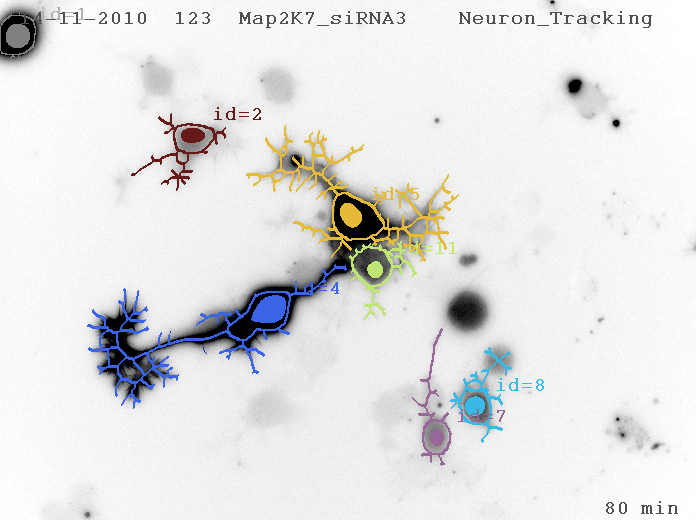
\includegraphics[width=60mm] {images/mv1_008.png} &
        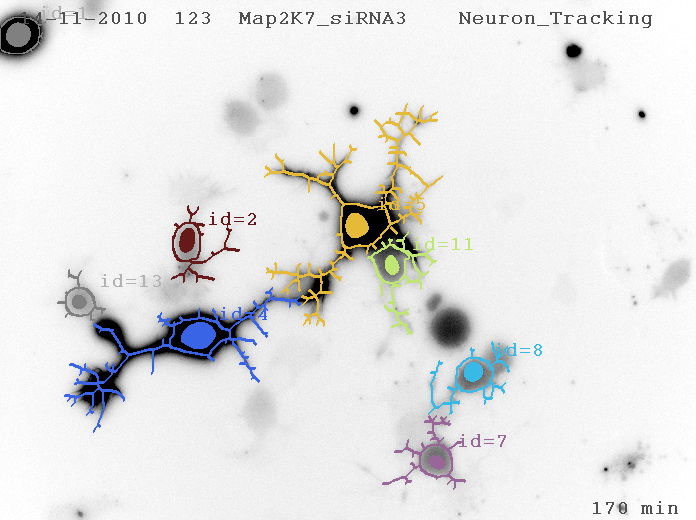
\includegraphics[width=60mm] {images/mv1_017.png}  &
        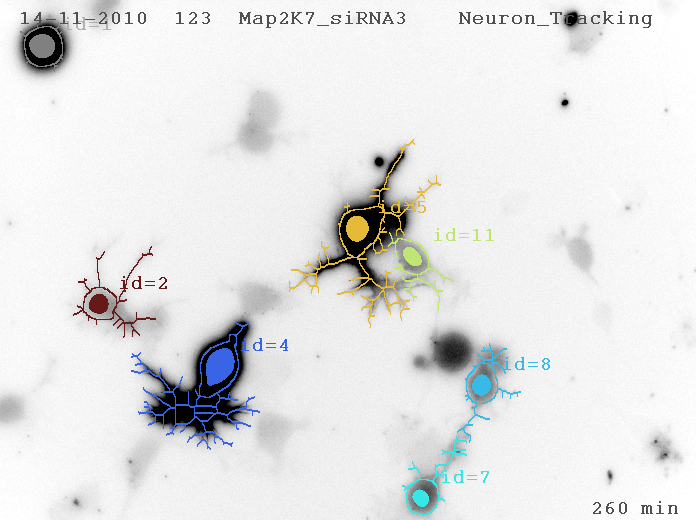
\includegraphics[width=60mm] {images/mv1_026.png} \\ [-.8ex]
        \hline \\ [-2.9ex]
       \end{tabular} 
      \begin{tabular}{@{\hspace{0mm}}c@{}c@{}|@{}c@{}c@{}|@{}c@{}c@{}}
        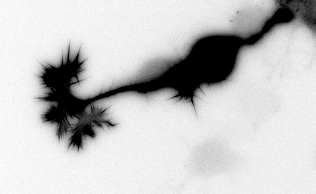
\includegraphics[width=30mm] {images/0_008.png} & 
        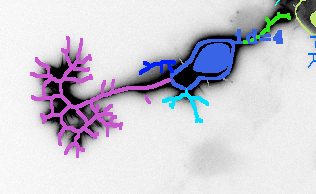
\includegraphics[width=30mm] {images/2_008_thick.png} & 
        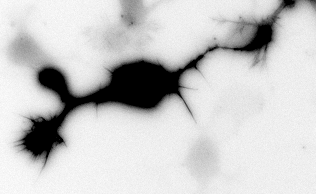
\includegraphics[width=30mm] {images/0_017.png} & 
	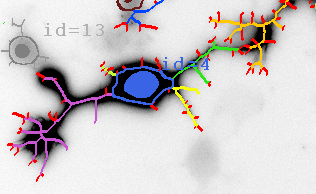
\includegraphics[width=30mm] {images/2_017_thick.png} & 
        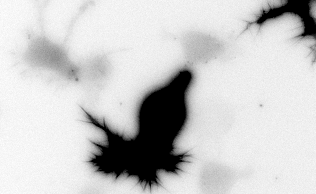
\includegraphics[width=30mm] {images/0_026.png} &
        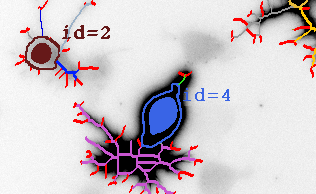
\includegraphics[width=30mm] {images/2_026_thick.png} \\ [-1ex]
	\multicolumn{2}{c}{\footnotesize $t = 80$ min} & 
	\multicolumn{2}{c}{\footnotesize $t = 170$ min} & 
	\multicolumn{2}{c}{\footnotesize $t = 260$ min} \\
      \end{tabular} 
    \vspace{-2mm}  
    \caption{\footnotesize Our approach tracks and segments the entire neuron. The top
        row contains results from an experiment with inhibited 
	MAP2K7 functions.    Tracked neurons are marked by a unique color and id.   
	Nuclei  are denoted  by  filled  ellipsoids, somata  as
        contours,  and neurites  as trees.   The bottom shows details
        from  above: the original  image on the left and  neurites
        marked with various colors on the right. Filopodia are marked in red. 
	Our  approach   performs  well  even  in  challenging
        situations where neurons appear in close proximity. Note: contrast has been 
	enhanced for visibility, faintly  stained
        cells are ignored for robustness.
	Video results can be viewed in our 
	\href{http://www.kev-smith.com/ISBI2013/}{online supplementary tables and videos}.
	}
    \label{fig:video}
\vspace{-4mm}
\end{figure*}
%----------------------------------------------------------------------------



%%----------------------------------------------------------------------------
%\begin{figure}[t]
%       \begin{tabular}{@{\hspace{0mm}}c@{}|@{}c@{}}
%        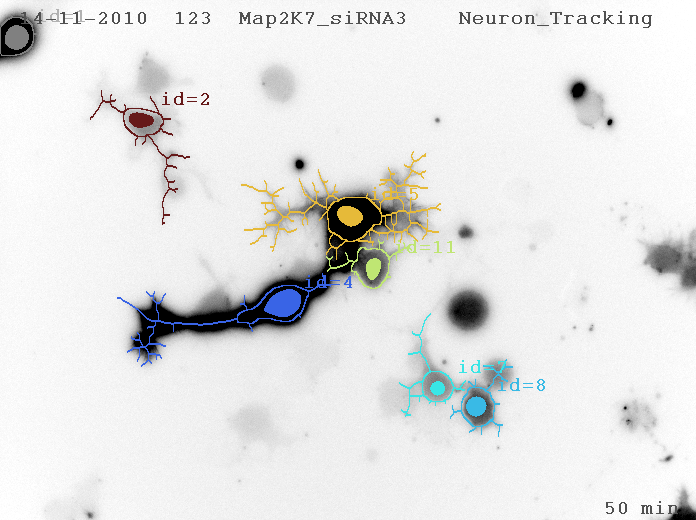
\includegraphics[width=45mm] {images/mv1_005.png}  &
%        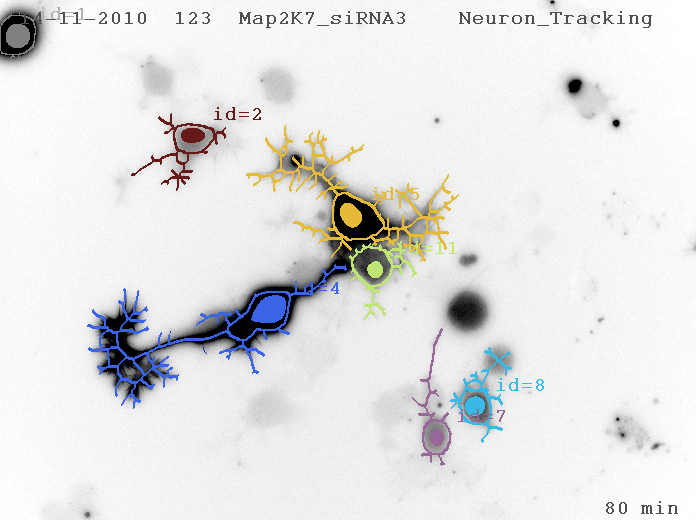
\includegraphics[width=45mm] {images/mv1_008.png} \\ [-.8ex]
%        \hline \\ [-2.6ex]
%        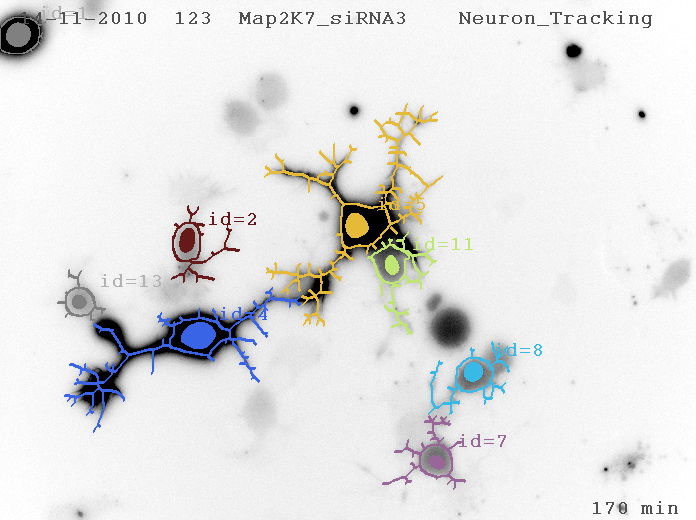
\includegraphics[width=45mm] {images/mv1_017.png}  &
%        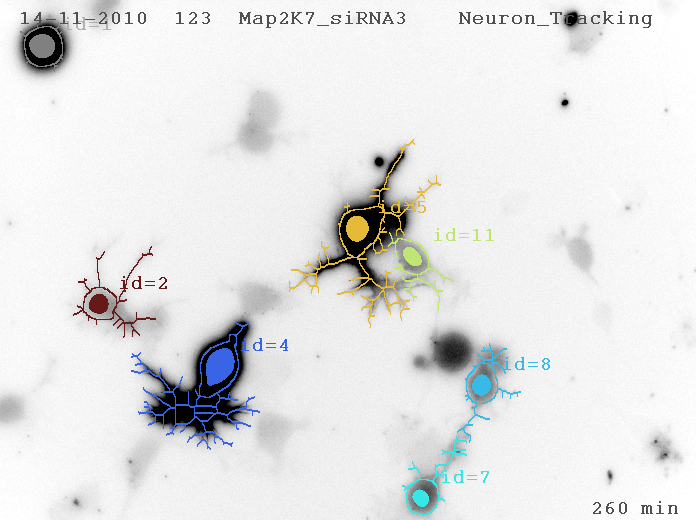
\includegraphics[width=45mm] {images/mv1_026.png} \\ [-.8ex]
%        \hline \\ [-2.9ex]
%       \end{tabular} 
%       
%      \begin{tabular}{@{\hspace{0mm}}c@{}c@{}c@{}c@{}}
%        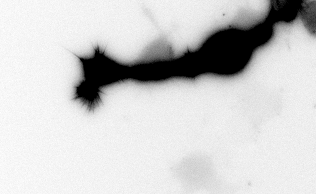
\includegraphics[width=22.5mm] {images/0_005.png} &
%        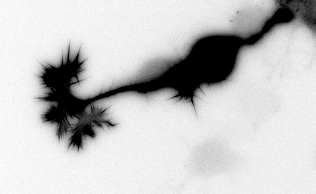
\includegraphics[width=22.5mm] {images/0_008.png} & 
%        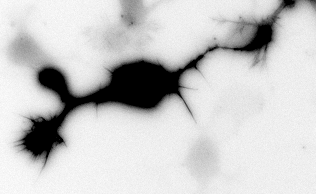
\includegraphics[width=22.5mm] {images/0_017.png} & 
%        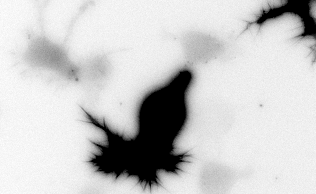
\includegraphics[width=22.5mm] {images/0_026.png} \\ [-1ex]
%        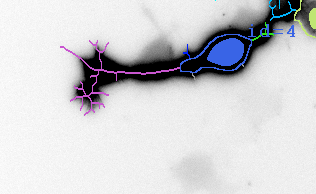
\includegraphics[width=22.5mm] {images/2_005.png} &
%        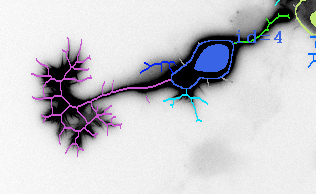
\includegraphics[width=22.5mm] {images/2_008.png} & 
%        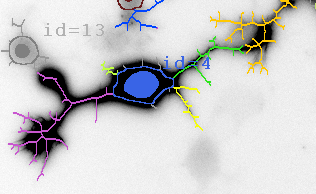
\includegraphics[width=22.5mm] {images/2_017.png} & 
%        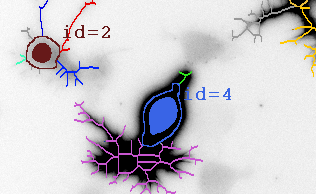
\includegraphics[width=22.5mm] {images/2_026.png} \\ [-1ex]
%        %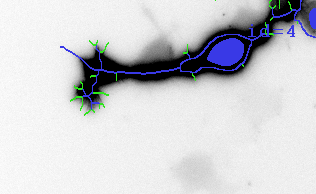
\includegraphics[width=22.5mm] {images/3_005.png} &
%        %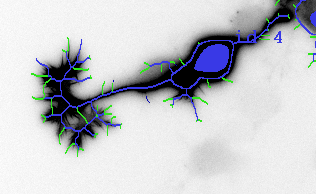
\includegraphics[width=22.5mm] {images/3_008.png} & 
%        %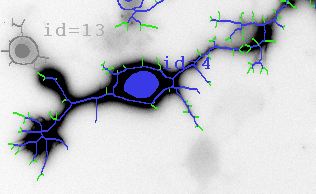
\includegraphics[width=22.5mm] {images/3_017.png} & 
%        %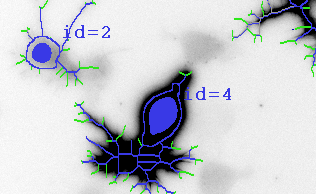
\includegraphics[width=22.5mm] {images/3_026.png} \\ [-1ex]
%        {\footnotesize $t = 50$ min} & 
%        {\footnotesize $t = 80$ min} & 
%        {\footnotesize $t = 170$ min} & 
%        {\footnotesize $t = 260$ min} \\ [-1ex]
%      \end{tabular}
%    \vspace{-2mm}  
%    \caption{ {\footnotesize {\it Neuron  Tracking Results.  } The top
%        two rows  contain frames from an experiment  where MAP2K7 gene
%        functions are inhibited.  For visibility we enhanced the image
%        contrast.  Tracked neurons are marked by a unique color and id
%        tag.   Nuclei  are denoted  by  filled  ellipsoids, somata  as
%        contours,  and neurites  as trees.   Bottom rows  show details
%        from  above: 1)  enhanced original  image 2)  tracked neurites
%        marked with a different colors. Our  approach   performs  well  even  in  challenging
%        situations where neurons appear in close proximity. Note: faintly  stained
%        cells are ignored for robustness.}}
%    \label{fig:video}
%\vspace{-6mm}
%\end{figure}
%%----------------------------------------------------------------------------



%======================================================================

%======================================================================
\begin{results}

%======================================================================
%======================================================================
\subsection{High content imaging of neurite outgrowth dynamics}
%======================================================================
To study neurite outgrowth dynamics, we used the mouse N1E-115 cell neuroblastoma cell line, that can be easily triggered to extend neurites by simple serum starvation and plating on the extracellular matrix protein laminin. To visualize soma and neurite morphology, we used a fusion of green fluorescent protein (GFP) with the F-actin binding peptide lifeact5. This provided high contrast on neurites and soma without excessive accumulation of fluorescence in the thick somata of differentiated N1E-115 cells, allowing for adequate imaging in N1E-115 cells by wide field microscopy (Figure 2a). For unambiguous cell identification, we also simultaneously labeled the nucleus with a mCherry fusion with a nucleus localization sequence (NLS), expressed from the same expression vector than Lifeact-GFP (Supplementary Fig.1a). We observed that transient expression of this construct did not affect neurite outgrowth in N1E-115 cells (Supplementary Fig.1b). To perturb different signaling pathways, we optimized a method to co-transfect the fluorescent marker and siRNAs simultaneously in cells, and observed efficient knockdown in response to knockdown of a panels of mRNAs (Supplementary note 1). To perform high content live cell imaging, we optimized our microscope for fast acquisition of multiple wells of a 24 well plate (Supplementary note 2). This allowed to acquire 240 fields of view in two channels across a 24-well plate with 12 minute time resolution for 20 hours. We performed different sets of experiments with 10 and 20x air objectives. Using 10 x objectives allowed for aquisition of a large field of view with typically 20 objects that could be consistently be observed for long time periods. The 20x objective allowed high resolution imaging of morphological features such as filopodia, but the moving cells often migrated out of the field of view resulting in loss of these objects. Typical 10x and 20x movies are shown (Supplementary movie 1 and 2). In these experiments, we tracked neuronal morphodynamics of differentiated cells that were replated on laminin, allowing to observe almost the whole neurite outgrowth process. We observed that illumination of neurons in the early phase of neurite outgrowth was toxic to the cells, leading to their death. We found that starting the observation process 3 hours post-plating, a time at which cells also had extended 3-4 neurites, allowed the cells to survive until the end of the imaging process.

\textcolor{red}{Describe verbally the neurite outgrowth process here ?}

%======================================================================

%======================================================================
%======================================================================
\subsection{Automated computer vision analysis of neurite ougrowth dynamics}
%======================================================================
To capture the dynamic neurite outgrowth trajectories of neurons in the native and perturbed state, we developed a computer vision pipeline that allowed to automatically segment and track the soma and neurites in each frame of the timelapse datasets. Our approach first detects nuclei and associated somata at each time step. The nucleus of each neuron is detected as a Maximally Stable Extremal Region (MSER)6 from the Cherry channel. [As shown in the supplementary note 3, this is more robust than adaptive thresholding.] Using the detected nuclei as seed points, a region-growing algorithm segments the neuron�s soma. Next, the implemented multi-objects tracking algorithm7 searches through the full set of nuclei and somata detections to extract the best K-shortest paths according to a similarity measure between two detections. The proposed similarity measure is derived from the Earth Mover�s Distance8 between the intensity histograms of the detected somata regions (in the supplementary note 3, we show that this distance provides a good tradeoff between efficiency and precision).  Neurons are detected and tracked at an accuracy of (TODO 95\%) (more than 2000 objects TODO); �Finally, the tracked somata are used to initialize a neurite segmentation and association algorithm based on shortest path computation and Voronoi tessellation. Comparison to manually annotated data demonstrates that �(URGENT TODO: crunch the numbers)�





\textcolor{red}{
Fethallah and Kevin can you please write a 10 line long, accessible paragraph that explains the segmentation procedure and the quantification of its efficiency in comparison with the manually annotated ground truth. We can add a supplementary note (Supplementary note 3) that describes the process in depth.
}
Can you please also sketch figure 2 that is dedicated to the segmentation process. This figure will show:
\begin{enumerate}
\item raw green and red images (it is the 1st figure in which we will show this). 
\item schematics of successive steps in the image segmentation.
\item A fully segmented time series of neurons as an example.
\item Some kind of efficiency evaluation in comparison with the manually annotated ground truth.
\end{enumerate}
Please then write another paragraph that explains the different static and dynamic features that are extracted.
\textcolor{red}{
Please sketch figure 3, which explains graphically how some static and dynamic features are extracted. You can represent some of the trajectories of one or two features over time. For this, you can use one of the presentation that Kevin once made. I would try to show a graph of a feature trajectory that is stochastic like the protrusion/retraction cycles of neurite outgrowth. This shows that we look at highly dynamic events, and thus illustrates the benefit of our approach. We can add a number of supplementary movies with different morphological features that are analyzed (soma, each new neurites). Please prepare also supplementary tables about the definition of features (supp tables 1 and 2). Then we also need a supplementary note that explain the format in which the morphodynamic history of each cell is explained.}

%======================================================================

%======================================================================
\subsection{To Riwal}
\begin{enumerate}
\item describe feature selection algorithms
\item validation of feature selection algorithm by mixing data from two perturb states
\item explain approaches to take into account siRNA noise
\end{enumerate}

%======================================================================

%======================================================================
\end{results}
%======================================================================

\bibliographystyle{naturemag}
\bibliography{biology,vision,ml}

%
%\begin{thebibliography}{1}
%\bibitem{Collinet10} No compound references -- only one source per reference.
%
%%\bibitem{dummy} Articles are restricted to 50 references, Letters to 30.
%%\bibitem{dummyb} No compound references -- only one source per reference.
%\end{thebibliography}


\begin{addendum}
 \item Put acknowledgements here.
 \item[Competing Interests] The authors declare that they have no
competing financial interests.
 \item[Correspondence] Phone: +41 61 267 22 03; Fax: +41 61 267 35 66; E-mail : \texttt{olivier.pertz@unibas.ch}.
\end{addendum}

%%
%% TABLES
%%
%% If there are any tables, put them here.
%%

\end{document}









%======================================================================

%% Example Figure commented
%FFFFFFFFFFFFFFFFFFFFFFFFFFFFFFFFFFFFFFFFFFFFFFFFFFFFFFFFFFFFFFFFFFFFFF
%\begin{figure}
%\caption{Each figure legend should begin with a brief title for
%the whole figure and continue with a short description of each
%panel and the symbols used. For contributions with methods
%sections, legends should not contain any details of methods, or
%exceed 100 words (fewer than 500 words in total for the whole
%paper). In contributions without methods sections, legends should
%be fewer than 300 words (800 words or fewer in total for the whole
%paper).}
%\end{figure}
%FFFFFFFFFFFFFFFFFFFFFFFFFFFFFFFFFFFFFFFFFFFFFFFFFFFFFFFFFFFFFFFFFFFFFF

%Figures
%Figure 1. Global pipeline to analyze neurite outgrowth morphodynamic phenotypes. (olivier and Ludo)
%Figure 2. Computer vision segmentation of neuronal morphodynamics feature extraction.
%(Fethallah and Kevin)
%Figure 3.  Description of morphodynamic features.
%(Fethallah and Kevin)
%Figure 4. Morphodynamic phenotype feature selection
%(Riwal)
%try to make a  series of schemes that explain the different steps in feature selection,
%vector distance, assessment of interplate and siRNA induced noise.
%
%Figure 5.  Morphodynamic phenotype description.
%(Riwal, Olivier, Ludo)
% this will consist of a color-coded map of the different features extracted for each gene perturbation, we will then focus on more specific aspects of what we learned.
%
% 
%Supplementary Figures.
%
%Figure S1. Experimental controls lifeact-GFP/NLS-mCherry reporter and siRNA transfection.
%(a) Structure of the Lifeact-GFP IRES NLS-mCherry expression vector. (b) Effect of Lifeact-GFP expression on neurite outgrowth.
%(ludo and olivier)
%
%
%Figure S2. Feature selection on synthetic data produced by mixing videos from different known sources to test the ability of the algorithm to appropriately identify different morphodynamic signatures (Riwal)
%
%
%
%?
%
%Supplementary tables.
%
%Table S1. Definition of static features.
%Table S2. Definition of dynamic features.
%
%
%
%?
%Supplementary notes
%
%Supplementary note 1. Description of RNA interference experiments.
%
%Olivier and ludo
%
%Supplementary note 2. Description of microscope setup used for high content acquisition.
%Olivier and ludo
%
%
%Supplementary note 3. In depth description of computer vision segmentation and evaluation of the method by comparison with ground truth.
%
%Fethallah and Kevin
%
%
%Supplementary note 4. Description of html format in which the cell trajectories are described
%
%Fethallah and Kevin
%
%?
%Supplementary movies.
%
%Supplementary movie 1. Representative timelapse movie of N1E-115 cells expressing the GFP-lifeact-IRES-NLS-mcherry construct with the 10x PlanApo objective.
%
%Supplementary movie 2. Representative timelapse movie of N1E-115 cells expressing the GFP-lifeact-IRES-NLS-mcherry construct with the 20x PlanApo objective.
%
%Supplementary movie 3.
%
%
%
%
%
% 
%References
%
%1.	B. Snijder, R. Sacher, P. Ramo et al., Nature 461 (7263), 520 (2009).
%2.	C. Collinet, M. Stoter, C. R. Bradshaw et al., Nature 464 (7286), 243 (2010).
%3.	M. Held, M. H. Schmitz, B. Fischer et al., Nature methods 7 (9), 747 (2010).
%4.	D. Loerke, Q. le Duc, I. Blonk et al., Science signaling 5 (231), rs5 (2012).
%5.	J. Riedl, A. H. Crevenna, K. Kessenbrock et al., Nature methods 5 (7), 605 (2008).

